% ==============================================================================
% PAGE 31: 3.2 SOLAR TRACKING MECHANISM - INTRODUCTION (Numbered Page 23)
% ==============================================================================
\subsection*{3.2) SOLAR TRACKING MECHANISM :}

\begin{center}
  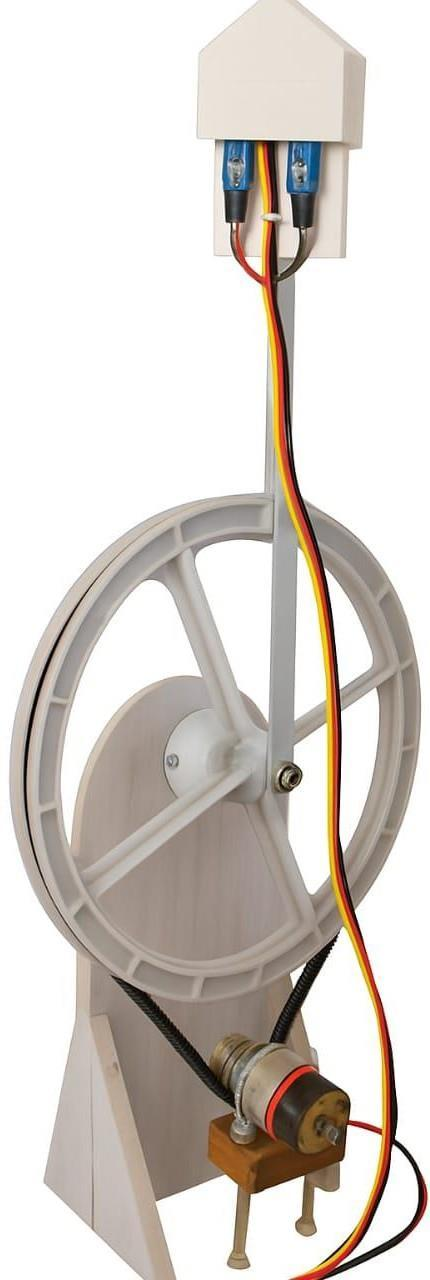
\includegraphics[width=45mm]{figures/fig15_solar_tracking_mechanism.jpg}
\end{center}

\subsubsection*{1. Introduction}
\noindent
\begin{spacing}{1.25}
{\fontsize{10.2}{15}\selectfont
The single-axis solar tracking mechanism is used to automatically rotate the parabolic dish from east to west to follow the sun's movement.\\[2.5mm]
It helps maintain maximum sunlight focus on the receiver throughout the day.\\[2.5mm]
The system works using LDR sensors, a PMDC motor, and a control circuit powered by solar energy.\\[2.5mm]
This automatic motion increases the overall efficiency and heat output of the solar water heater. It is a simple, low-cost, and effective method for improving solar energy utilization.
}
\end{spacing}
\clearpage
